\section{Phương pháp}

\subsection{Tiền xử lý và xây dựng từ vựng}

\begin{figure}[htbp]
    \centering
    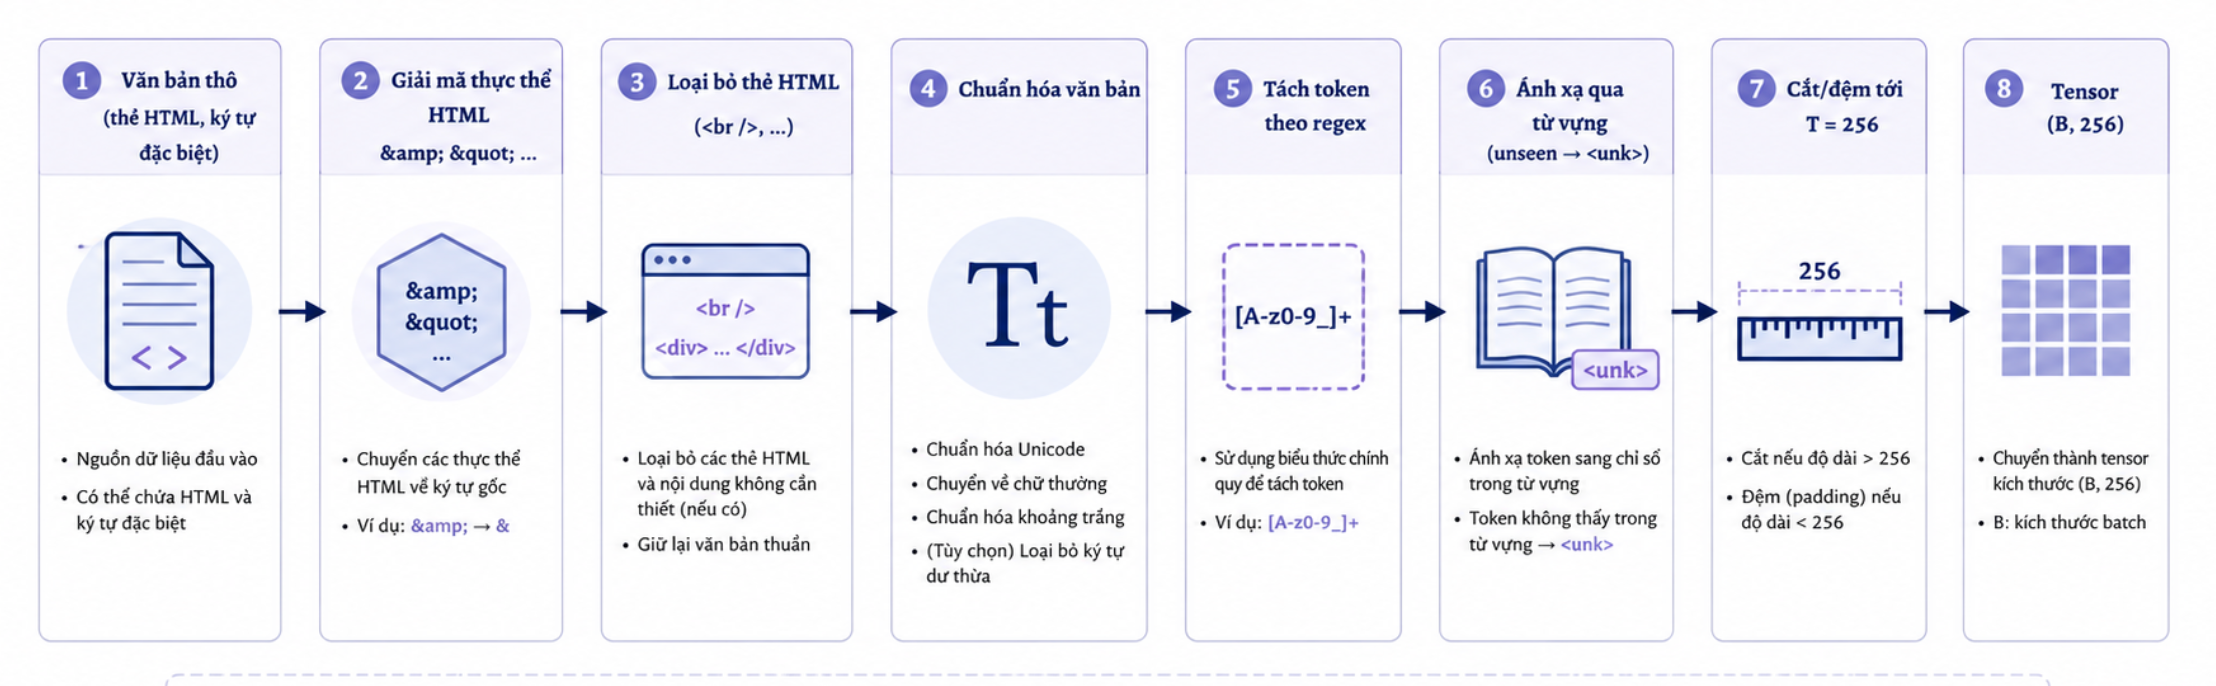
\includegraphics[width=\textwidth]{figures/data_processing.png}
    \caption{Quy trình tiền xử lý văn bản thô tới chuỗi token có độ dài cố định.}
    \label{fig:quy-trinh-tien-xu-ly}
\end{figure}

Quy trình tiền xử lý dữ liệu đầu vào bao gồm bốn bước tuần tự chặt chẽ: giải mã các thực thể HTML, loại bỏ hoàn toàn các thẻ HTML thông qua biểu thức chính quy, chuyển đổi toàn bộ văn bản về dạng chữ thường, và tiến hành \textit{tokenization} bằng biểu thức chính quy để giữ lại các ký tự chữ-số cùng dấu nháy đơn trong từ. Cách tiếp cận dựa trên \textit{rule-based} này đảm bảo tính xác định và khả năng tái lập cao của quy trình xử lý dữ liệu.

Không gian từ vựng của hệ thống được giới hạn nghiêm ngặt ở quy mô $10\,000$ token, bao gồm hai token đặc biệt là \texttt{<pad>} (gán chỉ số 0) và \texttt{<unk>} (gán chỉ số 1), tiếp theo là $9\,998$ từ xuất hiện phổ biến nhất xét theo tần suất xuất hiện trong tập huấn luyện. Một quyết định bắt buộc về mặt nguyên tắc thực nghiệm thống kê là tập từ vựng này chỉ được phép khởi tạo và khớp trên $22\,500$ mẫu của tập huấn luyện sau khi đã tách riêng tập kiểm định, tuyệt đối không sử dụng bất kỳ thông tin nào từ tập kiểm định hoặc tập kiểm thử . Mọi token không nằm trong danh mục từ vựng đã học từ tập huấn luyện sẽ được ánh xạ tự động về token \texttt{<unk>} khi xuất hiện ở các tập đánh giá. Nếu vi phạm nguyên tắc này, thống kê tần suất từ tập kiểm thử sẽ bị rò rỉ ngược vào không gian biểu diễn của mô hình (\textit{data leakage}), dẫn đến các kết quả đánh giá sai lệch và lạc quan hơn rất nhiều so với thực tế.

Cuối cùng, độ dài của chuỗi đầu vào được chuẩn hóa cố định ở ngưỡng $T = 256$ token; các văn bản dài hơn ngưỡng này sẽ bị cắt cụt và các văn bản ngắn hơn sẽ được lấp đầy bằng token \texttt{<pad>}. Ngưỡng cắt $256$ là kết quả của sự đánh đổi tối ưu giữa khả năng bao phủ phân phối độ dài thực tế (xấp xỉ $85\%$ số bài đánh giá trong tập dữ liệu có độ dài nhỏ hơn $T$) và chi phí tính toán tài nguyên của mạng hồi quy, vốn có độ phức tạp thuật toán được xác định ở mức $\mathcal{O}(B \cdot T \cdot d^2)$.

\subsection{Kiến trúc mô hình}

Mô hình tuân thủ chặt chẽ ràng buộc thiết kế ba tầng Embedding $\to$ GRU $\to$ Linear, với một tầng dropout chèn giữa pooled hidden state và lớp tuyến tính cuối nhằm phục vụ chính quy hóa. Sơ đồ tổng thể được trình bày ở Hình~\ref{fig:kien-truc-mo-hinh}.

\begin{figure}[htbp]
    \centering
    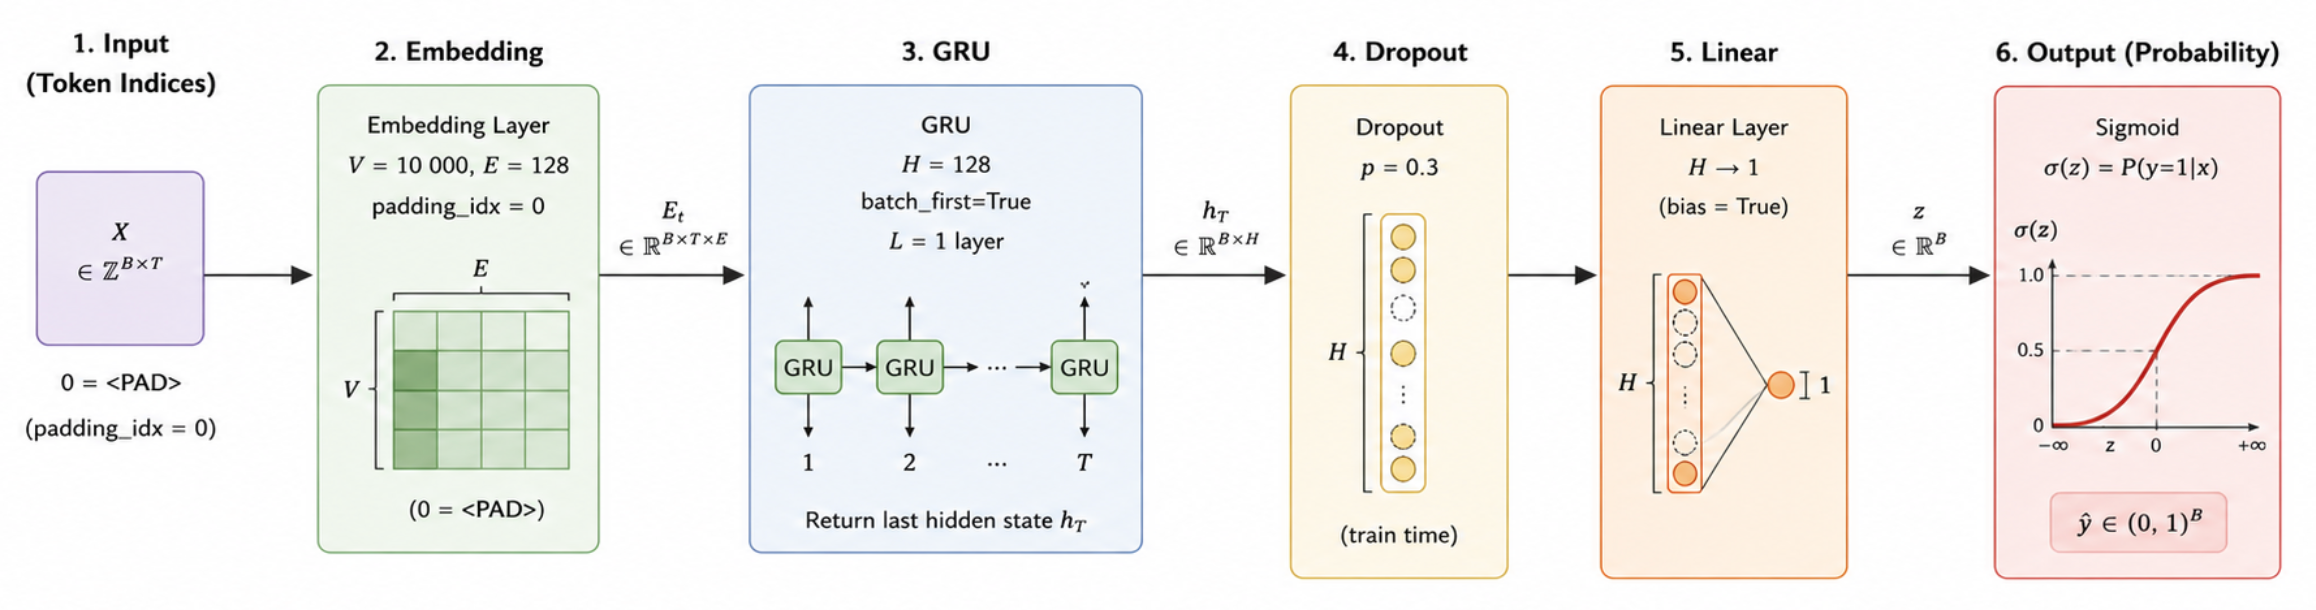
\includegraphics[width=\textwidth]{figures/gru_architecture.png}
    \caption{Kiến trúc mô hình GRU phân loại cảm xúc nhị phân.}
    \label{fig:kien-truc-mo-hinh}
\end{figure}

Trái tim của mô hình là phép cập nhật GRU. Với embedding đầu vào $x_t \in \mathbb{R}^E$ tại bước thời gian $t$ và trạng thái ẩn trước đó $h_{t-1} \in \mathbb{R}^H$, ba cổng được tính tuần tự như sau:
\begin{align}
r_t &= \sigma(W_{ir} x_t + b_{ir} + W_{hr} h_{t-1} + b_{hr}) && \text{(cổng đặt lại)} \\
z_t &= \sigma(W_{iz} x_t + b_{iz} + W_{hz} h_{t-1} + b_{hz}) && \text{(cổng cập nhật)} \\
n_t &= \tanh(W_{in} x_t + b_{in} + r_t \odot (W_{hn} h_{t-1} + b_{hn})) && \text{(trạng thái dự tuyển)} \\
h_t &= (1 - z_t) \odot n_t + z_t \odot h_{t-1} && \text{(trạng thái ẩn)}
\end{align}
trong đó $\sigma$ là hàm sigmoid và $\odot$ là tích Hadamard. 

Vai trò của hai cổng có thể được diễn giải như sau. Cổng đặt lại $r_t$ kiểm soát mức độ phụ thuộc của trạng thái dự tuyển $n_t$ vào trạng thái cũ; khi $r_t \to 0$, mô hình quên hoàn toàn quá khứ trong chiều đó, tương ứng với việc bắt đầu một mệnh đề mới hoặc một chủ thể mới trong câu. Cổng cập nhật $z_t$ thực hiện nội suy tuyến tính giữa hai cực: $z_t \to 0$ tương ứng với việc ghi đè hoàn toàn bằng candidate, $z_t \to 1$ tương ứng với việc giữ nguyên trạng thái cũ. Bằng cách cho phép gradient lan truyền gần như không suy giảm qua các bước thời gian mà $z_t$ gần $1$, giúp GRU bảo toàn tín hiệu cảm xúc trong các bài đánh giá dài, khắc phục hiện tượng vanishing gradient của RNN cổ điển.

Đếm tham số cho cấu hình mặc định ($V=10\,000, E=H=128$, một lớp) cho kết quả: tầng embedding chiếm $V \cdot E = 1\,280\,000$ tham số, tầng GRU chiếm $3(EH + H^2 + 2H) = 99\,072$ tham số (trong đó hệ số $3$ phản ánh ba cổng và thành phần $2H$ là độ lệch của input và hidden), lớp tuyến tính cuối chiếm $H + 1 = 129$ tham số. Tổng cộng mô hình có $1\,379\,201$ tham số có thể huấn luyện, trong đó tầng embedding chiếm khoảng $93\%$. Phân bố tham số được minh họa ở Bảng~\ref{tab:phan-bo-tham-so} — một dạng phân bố điển hình của các mô hình ngôn ngữ quy mô nhỏ và là một động cơ tự nhiên cho việc chính quy hóa mạnh ở tầng embedding.

\begin{table}[htbp]
\centering
\caption{Phân bố tham số huấn luyện theo tầng.}
\label{tab:phan-bo-tham-so}
\begin{tabular}{lrc}
\toprule
\textbf{Tầng} & \textbf{Số tham số} & \textbf{Tỉ lệ} \\ \midrule
Embedding ($V \times E$) & $1\,280\,000$ & $92,8\%$ \\
GRU ($3(EH + H^2 + 2H)$) & $99\,072$     & $7,2\%$  \\
Linear ($H + 1$)         & $129$         & $< 0,01\%$ \\ \midrule
\textbf{Tổng}            & $\mathbf{1\,379\,201}$ & $\mathbf{100\%}$ \\ \bottomrule
\end{tabular}
\end{table}

Một chi tiết kỹ thuật mang tính chính xác chứ không chỉ tốc độ là việc đóng gói chuỗi (\texttt{pack\_padded\_sequence}). Khi truyền vào GRU một mini-batch chứa các chuỗi có độ dài khác nhau, các vị trí padding ở cuối không nên được tham gia vào phép cập nhật trạng thái ẩn, vì ngay cả khi embedding tại đó bị buộc về $0$ thì các thành phần bias trong phép tính cổng vẫn làm nhiễu trạng thái cuối cùng. Đóng gói chuỗi cho phép GRU bỏ qua hoàn toàn các bước thời gian trên padding, mang lại trạng thái ẩn cuối cùng trung thực với phần thông tin có nghĩa của văn bản.

\subsection{Hàm mất mát và bộ tối ưu}

Do bài toán là phân loại nhị phân và mô hình xuất ra một logit duy nhất, hàm mất mát tự nhiên là binary cross-entropy. PyTorch hiện thực hóa nó dưới dạng softplus ổn định số học:
\begin{equation}
L_{\text{BCE}}(z, y) = \max(z, 0) - z \cdot y + \log(1 + e^{-|z|})
\end{equation}
dạng này tránh phép $\log(0)$ ngay cả khi $\sigma(z)$ bão hòa về $0$ hoặc $1$, nhờ đó loại trừ hoàn toàn hiện tượng NaN trong gradient.

Việc lựa chọn cấu hình một logit (kết hợp với \texttt{BCEWithLogitsLoss}) thay vì hai logit (kết hợp với \texttt{CrossEntropyLoss}) là tương đương về mặt toán học cho bài toán hai lớp: áp softmax lên vectơ hai logit $(z_0, z_1)$ rồi lấy log của xác suất tương ứng với lớp đúng đồng nhất với BCE trên logit chênh lệch $z = z_1 - z_0$. Cấu hình một logit có lợi thế thực dụng ở chỗ giảm một nửa tham số ở lớp đầu ra và loại bỏ phép softmax không cần thiết tại thời điểm suy luận.

Bộ tối ưu là Adam (Kingma và Ba, 2015) với các siêu tham số chuẩn $\beta_1 = 0.9, \beta_2 = 0.999, \epsilon = 10^{-8}$. Cập nhật của Adam được mô tả bởi hệ phương trình:
\begin{align}
m_t &= \beta_1 m_{t-1} + (1 - \beta_1) g_t \\
v_t &= \beta_2 v_{t-1} + (1 - \beta_2) g_t^2 \\
\hat{m}_t &= \frac{m_t}{1 - \beta_1^t} \\
\hat{v}_t &= \frac{v_t}{1 - \beta_2^t} \\
\theta_t &= \theta_{t-1} - \frac{\eta}{\sqrt{\hat{v}_t} + \epsilon} \hat{m}_t
\end{align}

Adam là lựa chọn phù hợp với mô hình hồi quy vì hai lý do mang tính bản chất. Thứ nhất, gradient của các nhóm tham số trong một mô hình GRU có biên độ chênh lệch lớn: gradient của embedding thưa và có fan-out lớn, gradient của các ma trận hồi quy dày và có biên độ trung bình, gradient của lớp đầu ra dày và có biên độ nhỏ. Phép chuẩn hóa theo căn bậc hai của moment bậc hai trong công thức cập nhật của Adam tự động cân bằng biên độ giữa các nhóm này, trong khi một learning rate cố định kiểu SGD sẽ hoặc làm các embedding hiếm không bao giờ được cập nhật đáng kể, hoặc làm lớp đầu ra bùng nổ. Thứ hai, lan truyền ngược qua thời gian trên $256$ bước tạo ra gradient có phương sai cao; trung bình động mũ $m_t$ giảm độ ồn của hướng cập nhật một cách tự nhiên, không cần giai đoạn khởi động dài như momentum cổ điển.

\subsection{Huấn luyện và chính quy hoá}

Mỗi epoch gồm một lượt quét tập huấn luyện ở chế độ huấn luyện bao gồm các bước \textit{forward pass}, tính toán hàm mất mát BCE, \textit{backward pass}, cắt gradient theo chuẩn $\ell_2$ ở ngưỡng $1,0$, cập nhật trọng số bằng thuật toán Adam, và một lượt quét tập kiểm định ở chế độ đánh giá không cập nhật tham số. Bốn đại lượng cốt lõi bao gồm \textit{train loss}, \textit{train accuracy}, \textit{val loss}, và \textit{val accuracy} được ghi lại một cách hệ thống theo từng epoch. Trong đó, kỹ thuật cắt gradient là bắt buộc khi huấn luyện các mạng hồi quy RNN bằng Adam, đặc biệt là ở các mức \textit{learning rate} cao, nhằm triệt tiêu hiện tượng bùng nổ gradient.

Để chống lại hiện tượng \textit{overfitting}, ba kỹ thuật \textit{regularization} mạnh mẽ được áp dụng đồng thời, vượt qua các yêu cầu tối thiểu của đề bài. Đầu tiên, \textit{dropout} với xác suất $p=0,3$ được đặt ngay sau trạng thái ẩn cuối cùng và trước lớp tuyến tính; đây là vị trí có mật độ thông tin tập trung cao nhất, giúp việc ngắt ngẫu nhiên các liên kết có hiệu lực mạnh nhất và có thể được diễn giải lý thuyết như một phép xấp xỉ \textit{ensemble} Bayesian (Gal và Ghahramani, 2016). Thứ hai, kỹ thuật \textit{weight decay} với hệ số $\lambda=10^{-5}$ được tích hợp trực tiếp vào quá trình tối ưu của Adam, tương đương với việc bổ sung một số hạng phạt bậc hai $\frac{\lambda}{2}\|\theta\|_2^2$ vào hàm mất mát để kéo các giá trị trọng số về gần góc tọa độ. Cuối cùng, cơ chế \textit{early stopping} với giá trị \textit{patience} bằng 3 đóng vai trò giới hạn dung lượng hiệu dụng của mô hình tại điểm mà \textit{val loss} đạt giá trị nhỏ nhất, từ đó đạt được sự đánh đổi giữa chệch và phương sai gần như tối ưu (Goodfellow và cộng sự, 2016).